\documentclass[11pt,oneside]{article} % for sharing

\usepackage{amsmath}
\usepackage{array}
\usepackage{caption}
\usepackage{placeins}
\usepackage{graphicx}
\usepackage{subcaption}
\usepackage{longtable}
\usepackage{setspace}
\usepackage{booktabs}
\usepackage{chngpage}
\usepackage[style=authoryear-comp]{natbib}
\bibpunct{(}{)}{,}{a}{}{;} 
\usepackage{url}
\usepackage{nth}
\usepackage{authblk}
\DeclareRobustCommand{\VAN}[3]{#2} 
% end preamble
%-------------------------------------------

\begin{document}

\title{Domains of application for the demographic time framework}

\author[1]{Tim Riffe\thanks{riffe@demogr.mpg.de\\ ~~~~(author order tbd)}}
\author[2,3]{Jonas Sch{\"o}ley}
\author[2,3]{Francisco Villavicencio}
\affil[1]{Max Planck Institute for Demographic Research}
\affil[2]{University of Southern Denmark}
\affil[3]{Max-Planck Odense Center on the Biodemography of Aging}

%\author{[Authors]}


\maketitle

\begin{abstract}
The demographic time framework defines the time-space for birth-death processes
that produce overlapping lifecourses. The framework is generally applicable to
any domain where population-level variation occurs over time and within ``life''. Since the
framework is an abstraction, both intuitively coherent, but not
necessarily obvious to translate into applications, we here offer a potluck of
suggested applications in a variety of domains, both within and outside demography.
Application domains include subfields of human demography focusing on particular transitions, stages of the life course, or special sub populations (prisoners, athletes, and professors), but also applications to non-human species, natural phenomena, and artificial objects.
\end{abstract}

*This is a very green paper for us at this point, but we expect to have a full
manuscript well before the final upload deadline.*

\section*{Background}
%Since change and process can only unfold in time, time is essential to all
%scientific inquiry. That events and change can be placed on a timeline, whether
% explicit chain reactions, a gradual unfolding of argumentation, a trajectory of growth or metabolism, or a population mean level
%of some health metric, 

%In many applications of human demography, time-to-event is inferred rather than
%measured directly

A singular relationship unites six distinct measures of demographic time:
chronological age (A), period (P), birth cohort (C), thanatological age (T,
also known as time-to-death), death cohort (D), and lifespan (L). Together,
these time measures define a time-space in three dimensions. The set of six
time measures also contains four three-member identities, each of which
tesselates to form a plane, or characteristic diagram. These identities are the
well-known APC identity, as well as the TPD, LCD, and TAL identities. A
fuller description about how these identities and diagrams relate, as well as an
example about how the time framework might guide scientific inquiry is given in
\citet{rsv2015}. In this paper, we intend to provide a diverse set of potential
uses of said time framework.


\section{Applications}

Although its original description was
motivated by the study of health patterns over the human lifecourse, where
complete human lifespans define the lifecourse boundary, this need not be the
case. The only empirical application given thus far has dealt with late-life
morbidity patterns \citep{riffe2015ttd}, and in this example the maximum human
lifespan sets the space boundary. While
this usage case is useful as a heuristic, and for qualifying morbidity comparisons or guiding morbidity projections
\citep{vanRaalte2015HLE}, it is also clear that providing more
examples of applications would help illustrate the transportability of the
framework and help guide other researchers in exploring its uses. For this
reason, we here aim to provide as diverse-as-possible set of applications in
different domains of inquiry. The domains that we aim to cover range from
standard human demography, medical research, special sub-populations defined by
variable points of entry and exit, biology, the so-called hard sciences, and
engineering. With such a wide variety of application domains, this treatment
will be neccesarily brief with respect to each, in most cases consisting in
sketches of potential analyses that we think would be feasible, but that we do
not have the data or expertise to carry out rigorously ourselves. For others, we
work up some exploratory results given novel perspectives on data already
available. 

Part of the motivation for hashing out such a range of suggested applications is
the common observation that time-to-death and age-at-death are unknown for
living persons. This invites the observer to question the
usefulness of the framework. In the first instance, the framework proves its
utility even under this limitation, as the late-life health patterns of the
deceased are the best and closest reference for the living. In other contexts,
adopting different time perspectives may reveal robust and meaningful features
of a process that chronological age patterns or even Lexis-surfaces fail to
reveal. Further, ``life lines'' in the population modeled need not cover the
full duration of a human life, and therefore might not succumb to impatience.
In an extreme, we posit novel patterns in the growth and reproduction of
bacteria, the lives of which are very short, and fully observable. Patterns in
such timescales may be reproduced at will in the laboratory, and if structured
by time since birth and time until death (or between well-defined stages) may be
treated as reference standards; as nuanced descriptions of the lifecourse of bacteria. Human gestation presents a duration window several orders of
maginitude longer, and also conformable to the TAL diagram. For human pregnancy,
time since conception or implanation, time until parturition, and duration
of gestation complete the TAL identity. These rich time measures may be used to
structure data describing the development in the fetus, placenta, or mother. If
patterns are based on a large and representative sample, standards
may be developed to provide a new perspective on prenatal demography.

Examples that will be included as this paper progresses are included in
outline format in what follows. These include novel time-perspectives on
demographic topics including birth-spacing, in-utero development, health
measures, migration, and labor force demography. Special population applications
will include examples from baseball player careers, recidivism or prison
populations, and professor populations. Applications in non-human demography
will come from bacterial growth and reproduction trajectories and a yet-to-be
chosen industrial item, such as automobiles.

All examples to be provided here are decidedly visual in nature, and this only
represents the first step in a complete analysis: that of pattern detection of
phenomena. Suggested posterior analyses might include the development of
synthetic indicators that better capture and are sensitive to patterns in data.

\section{Human demography}
The human lifecourse may be treated as a whole, or segmented into shorter
durations with well-defined starting and ending points. 

	\subsection{Reproduction}
	
		\subsubsection{Birth spacing}
		\FloatBarrier
		Table~\ref{tab:spacing} lists a selection of birth-spacing time measures that
		may be used to structure data and thereby uncover presently hidden patterns.
		The patterns that may be uncovered by structuring data in this way are not
		births, per se, since birth events define the bounds of the time-space, but
		rather other behaviors, or health measures that may vary within birth
		intervals. This may include, e.g., miscarriages, or it could be a variable
		seemingly beside the point, but whose patterns are nonetheless conditioned on
		birth-spacing.
		
		\begin{table}[h!]
		\caption{Some birth spacing time measures and corresponding time identities.}
	    \label{tab:spacing}
		\begin{tabular}{lc}
		Time measures & Identity \\ \hline
		Time since birth i, time until birth i+1, interval & TAL\\
		Time since birth i, year of birth i, year & APC\\
		Time until birth i+1, year, year of birth i+1 & TPD\\
		birth interval, year of birth i, year of birth i+1 & LCD
		\end{tabular}
		\end{table}
		
		Note that Table~\ref{tab:spacing} does not include mothers' absolute age, but
		it captures the interval period as a complete space. However, age at birth i
		may be used to condition any of the aforementioned surfaces, for instance.
		
		\subsubsection{In-utero development}
		
		Many routine measurements are taken by gynecologists that may be used to
		\textit{fill} the TAL plane defined by time since conception, time until
		parturition, and duration of gestation. Surely, each of these measures is a reasonable and
		complementary way of structuring the health and development of either fetus,
		placenta, or mother (or particular organs). We intend to seek data as provided
		by a common smart-phone app used by mothers in the prenatal period, in order
		to mock up some prenatal TAL surfaces, details tbd. 
		
		For the present, Figure~\ref{fig:prenat}
		provides sketch of how a prenatal diagram or surface is organized. This figure
		resembles a Lexis diagram, in a certain way, but the time coordinates are
		different. In this diagram, conception ocurrs somewhere on the left axis, and
		birth on the bottom axis. Various standard term categories are highlighted in
		the diagram. Such gestational duration categories are assigned after birth,
		naturally. However, if a large number of prenatal trajectories with
		respect some some variable were recorded, we could fill this diagram with
		quantitative information. Depending on the characteristic measured, a surface
		could yield horizontal, vertical, downward-right diagonal, or even
		upward-right diagonal gradients (or striations) of variation.
				
		\begin{figure}
		\caption{Mock-up of a prenatal diagram}
		\label{fig:prenat}
		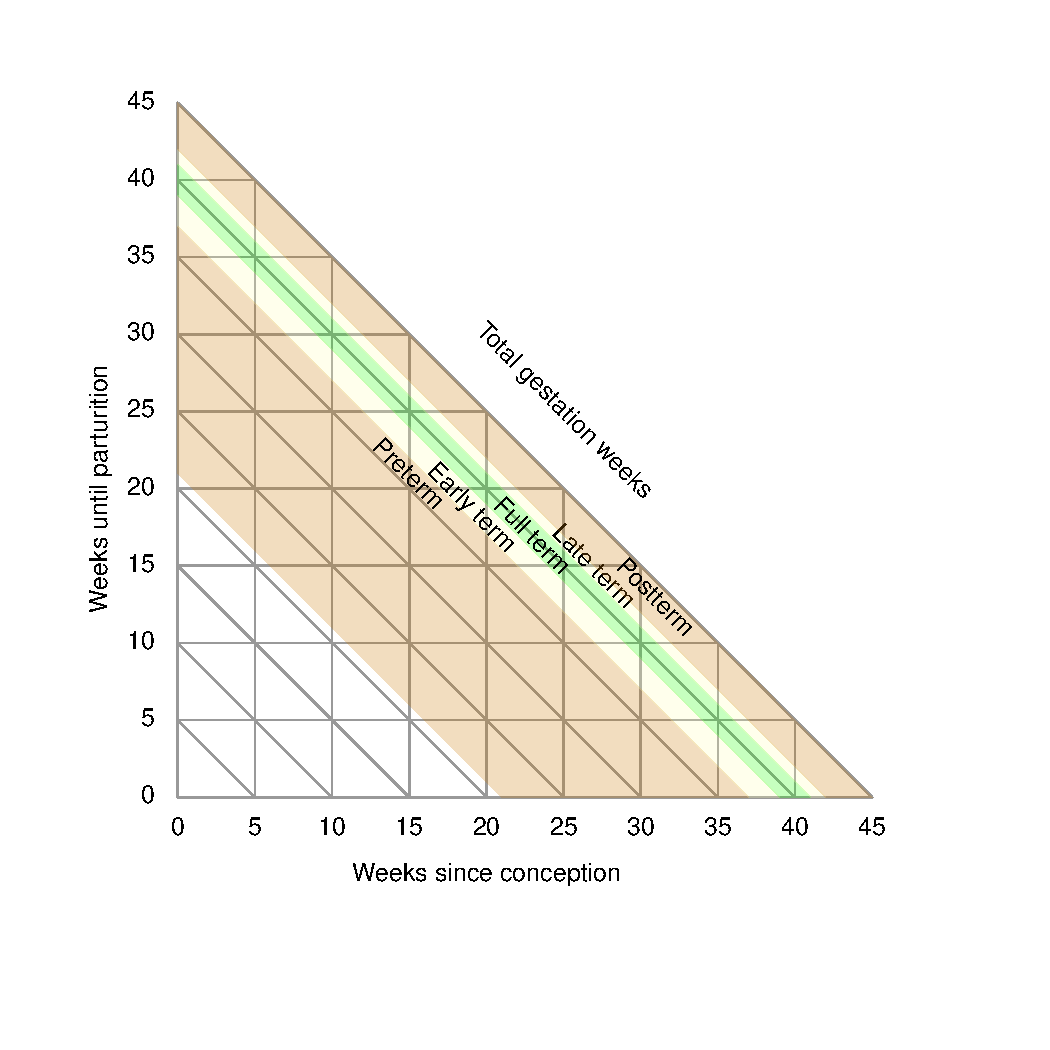
\includegraphics[scale=.8]{Figures/PrenatalDiagram.pdf}
		\end{figure}
		
		Table~\ref{tab:prenat} provides a fuller set of potential identities that may
		pertain to the prenatal period. Note the lack of maternal age.
		We suggest that this and other ``anchoring'' time variables may be used to
		condition surfaces in small multiples.
		
		\begin{table}[h!]
		\caption{Prenatal time measures, and corresponding time identities.}
	    \label{tab:prenat}
		\begin{tabular}{lc}
		Time measures & Identity \\ \hline
		Time since conc/impl, time until parturition, total gestation & TAL\\
		Time since conc/impl, calendar time, time of conc/impl & APC\\
		Time until parturition, calendar time, time of parturition & TPD\\
		total gestation, time of conc/impl, time of parturition & LCD
		\end{tabular}
		\end{table}
		
		\FloatBarrier
	\subsection{Health}
		
		Health measures may be modeled using prevalence or incidence-based models. At
		this time we have estimated measures of prevalence by birth cohort,
		time-until-death, and chronological age, as estimated from the U.S.
		\citet{HRS} \citep{riffe2015ttd}. Much variation in prevalence in the HRS
		morbidity measures is with respect to time-to-death, although
		chronological age is not insignificant, and there are a few other patterns as
		well. We have not studied what produces time-to-death patterns. Certainly
		time-to-death cannot \textit{cause} such patterns, since causes must precede
		effects. Such patterns may be produced in a mechanical way by, for instance, a
		series of health states that, once triggered, implied successive
		intensification (chronological) coupled with rapid
		increases in the risk of death. Ergo, a chronological incidence pattern could
		produce a thanatological prevalence pattern in a very intuitive way. However,
		estimating said incidence rates could bring its own difficulties, as could
		projecting them. Whether to model using prevalence or
		incidence is a tradeoff of convenience. We do not know if time-to-death patterns in incidence exist
		or not, but these are also possible.
	
	\subsection{Labor force demography}
	Time measures
	\subsection{Special subpopulations}
		\subsubsection{Professors}
		There are many ways to temporally structure the various stages of academia,
		but here we focus just on the process of acheiving tenure, which conforms to
		the six demographic time dimensions. If article submissions are the chosen
		metric, there will clearly be effects by time-since hire, period, hire cohort,
		tenure cohort (translation of death cohort), and duration under consideration, 
		and most especially time-until-decision. Data tbd, but this does seem
		tractable.
		
		
		\subsubsection{Prisoners (or recidivism)}
		Presumably health and behaviors vary both by
		time since entry and time until release, and certainly by duration of
		time served, for prison populations. Policy effects manifest as period
		effects. Time of entry and time or release may also mark the prisoner in
		various ways. Therefore, plausibly these translations of the six time measures
		could all be important time-structuring variables for prison populations. We
		aim to produce a small empirical example for this subsection as well, data
		source tbd.
		
		\subsubsection{Athletes}
		The empirical sports example we will provide in the full manuscript is based
		on rich data produced about Major League baseball players in the United States
\citep{Lahman}, which is structured in such as way as to easily conform with the
demographic time framework. Specifically, this database provides not only birth
and death (where applicable) dates of major league players, but also season
statistics. For the exploratory analysis begin, we specifically look at
pitching statistics as a function of time since debuting and time until retiring
from professional play, thereby implying the third time dimension of career
length. This particular setup is an event-history translation of the TAL
diagram.
\section{Non-human demography}	
	\subsection{Bacterial growth}
	We are working together with some lab-members that are producing rich data on
	bacterial cohorts, and expect to produce some novel
	time-structured visualizations of these as well, following the demographic time
	framework.
		
	\subsection{Industrial item (tbd)}
	
\section{Discussion}
Probably worth talking about statistical inference here.



\singlespacing
\bibliographystyle{plainnat}
  \bibliography{references} 

\end{document}